\documentclass[%
 aip,
% jmp,
% bmf,
% sd,
% rsi,
cp,  % Conference Proceedings
 amsmath,amssymb,%nobibnotes,
% preprint,%
 reprint,%
%author-year,%
%author-numerical,%
]{revtex4-2}

\usepackage{graphicx}% Include figure files
\usepackage{dcolumn}% Align table columns on decimal point
\usepackage{bm}% bold math
%\usepackage[mathlines]{lineno}% Enable numbering of text and display math
%\linenumbers\relax % Commence numbering lines

\usepackage[utf8]{inputenc}
\usepackage[T1]{fontenc}
%% Loads a Times-like font. You can also load
%% {newtxtext,newtxtmath}, but not {times}, 
%% {txfonts} nor {mathtpm} as these packages
%% are obsolete and have been known to cause problems.
\usepackage{mathptmx} 

\usepackage{physics}
\usepackage{tikz}
\usetikzlibrary{quantikz2}

\usepackage{amsthm}
\usepackage{subcaption}



\newcommand{\Q}{\mathbb{Q}}
\newtheorem{definition}{Definition}

\begin{document}

\title{Investigating Locality in Quantum Systems}% Force line breaks with \\

\author{Aditya K. Rao} % Write as First name Surname
 \email{adi.rao@mail.utoronto.ca}
%\author{Author's Name}%
% \email{second.author@institution.edu.}
\affiliation{
University of Toronto, 60 St. George Street, Toronto, Ontario M5S 1A7, Canada% Force line breaks with \\ if necessary
}

%\author{Another's Name}
% \email{third.author@anotherinstitution.edu}
%\affiliation{%
%Second institution and/or address% Force line breaks with \\ if necessary
%}%
%\affiliation{You would list an author's second affiliation (if applicable) here.}

\date{\today} % It is always \today, today, but any date may be explicitly specified
              % Not printed for conference proceedings

\begin{abstract}
    One of the key mysteries of quantum mechanics is the apparent faster-than-light communication between entangled particles. This was one of the qualms highlighted by Einstein, Podolsky, and Rosen in their famous EPR paper. Here, the locality of quantum systems and quantum mechanics is analyzed with reference to the phenomena of quantum teleportation. It is found that while information appears as though it is propagating nonlocally, in reality it can be explained using a local theory. The ideas of a nonlocal correlation and nonlocal information must be separated. Particularly, the concept of locally hidden or inaccessible information within subsystems of a wider quantum system is explained. Furthermore, it is shown that while some hidden-variable theories are proposed, they are not experimentally conclusive and do not provide a complete or better explanation of quantum mechanics.
    %\textcolor{red}{Edit Abstract}
\end{abstract}

\maketitle

\section{Introduction}
    The locality of quantum systems is itself curious and, in certain cases, ambiguous. In 1949 Einstein, Podolsky, and Rosen raised important questions as to whether quantum mechanics was complete as a local theory. In the EPR experiment \cite{epr}, quantum mechanics appeared to violate causality and special relativity. However, experimentally the theory of quantum mechanics still works. For example, consider quantum teleportation \cite{teleport} with qubit states being teleported\footnote{In this specific example the Bell state mediating the teleportation was created prior to being distributed to a satellite in low-Earth-orbit.} as far as 1200 \ km at $82\pm 1 \%$ fidelity \cite{long_range_teleport}. Under careful scrutiny, one can verify that these seemingly instantaneous nonlocal interactions are truly still local \footnote{The locality in this paper is Einsteinian locality (causality)}.
    This article assumes a familiarity with core aspects of quantum mechanics such as pure states, entangled states, and superposition/wave functions. Furthermore, a na{\"i}ve understanding of computer science, quantum computing, and information theory is recommended.
\section{Key Definitions and Concepts}
    \subsection{Defining Locality}
    %\subsection{Definition of Locality in this Paper}
        Later referred to as Einstein's locality, a local interaction has to do with the idea of causality. Definition 1 was adapted from a talk by Alain Aspect \cite{aspect}. Essentially, any interaction faster than light (space-like separated) is nonlocal and violates Einstein's locality.
        \begin{definition} \label{def:local} 
            A local interaction is one in which two events happen at the same point in spacetime [Fig. 1(a)]. Locality is also preserved in time-like separated events [Fig. 1(b)]. Any other interaction [Fig. 1(c)] is nonlocal.
        \end{definition}
        \begin{figure}[ht]
            \centering
            \begin{subfigure}[t]{0.30\textwidth}
            \centering
            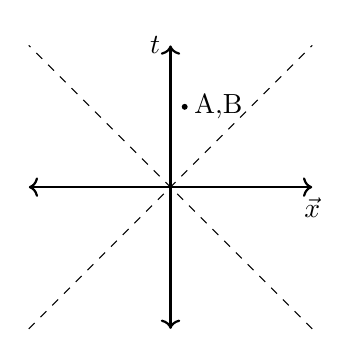
\begin{tikzpicture}[scale=0.6]
                \draw[thick, <->] (-3,0) -- (3,0)node[anchor=north]{$\vec{x}$};
                \draw[thick, <->] (0,-3) -- (0,3)node[anchor=east]{$t$};
                \draw[dashed] (-3,-3) -- (3,3);
                \draw[dashed] (3,-3) -- (-3,3);

                \filldraw (0.3,1.7)node[anchor=west]{A,B} circle (0.05);
            \end{tikzpicture}
            \caption{Two events/interactions at the same spacetime location are \textit{local}.}
            \label{fig:light-cone-l}
            \end{subfigure}
            \begin{subfigure}[t]{0.30\textwidth}
                \centering
                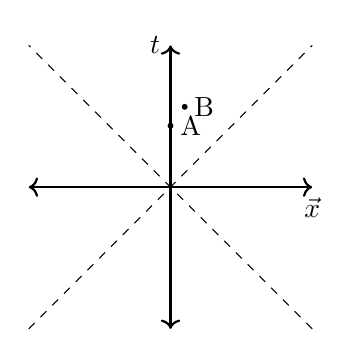
\begin{tikzpicture}[scale=0.6]
                    \draw[thick, <->] (-3,0) -- (3,0)node[anchor=north]{$\vec{x}$};
                \draw[thick, <->] (0,-3) -- (0,3)node[anchor=east]{$t$};
                \draw[dashed] (-3,-3) -- (3,3);
                \draw[dashed] (3,-3) -- (-3,3);

                \filldraw (0.3,1.7)node[anchor=west]{B} circle (0.05);
                \filldraw (0,1.3)node[anchor=west]{A} circle (0.05);
                %\draw (0,1.3) circle (0.7);
                %\draw (0.8,1.3)node[anchor=west]{bubble of radius $ct$};
                \end{tikzpicture}
                \caption{Two time-like events separated by a distance \textit{preserve Einstein's locality condition}.}
                \label{fig:light-cone-tl}
            \end{subfigure}
            \begin{subfigure}[t]{0.3\textwidth}
                \centering
                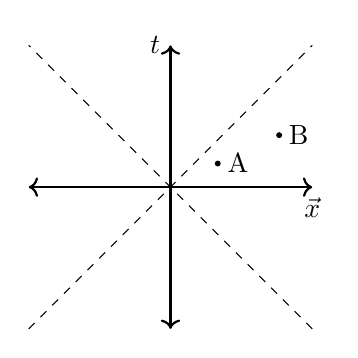
\begin{tikzpicture}[scale=0.6]
                    \draw[thick, <->] (-3,0) -- (3,0)node[anchor=north]{$\vec{x}$};
                    \draw[thick, <->] (0,-3) -- (0,3)node[anchor=east]{$t$};
                    \draw[dashed] (-3,-3) -- (3,3);
                    \draw[dashed] (3,-3) -- (-3,3);

                    \filldraw (2.3,1.1)node[anchor=west]{B} circle (0.05);
                    \filldraw (1,0.5)node[anchor=west]{A} circle (0.05);
                    %\draw (0,0.5) circle (0.7);
                    %\draw (0.8,0.4)node[anchor=west]{bubble of radius $ct$};
                \end{tikzpicture}
                \caption{Two space-like separated events are \textit{nonlocal}.}
                \label{fig:light-cone-sl}
            \end{subfigure}
            
            \label{fig:light-cone}
            \caption{Causality in different contexts}
        \end{figure}


    \subsection{Quantum Circuit Notation}
        This section serves as a brief overview of how to read a quantum circuit and the basic gates used in this paper. Quantum circuits are a method of visualizing the interactions on a qubit over time.  Time in circuits propagates from left to right. Each qubit is referred to as $\Q_n$ where $n$ is the index of the qubit. Qubits are indexed from \textit{bottom to top} in circuit diagrams and \textit{right to left} in Dirac notation. In Fig. 2(c), the control qubit is $\Q_0$ and the target qubit is $\Q_1$. Quantum gates such as $\hat{H}, \hat{X}, \hat{Y}, \hat{Z}, \ \text{and} \ \hat{U}$ represent local unitaries that are all Hermitian. In the computation basis, otherwise known as a \texttt{spin-1/2} system $\left(\ket{0}, \ket{1}\right)$, these are all represented as $2\times 2$ matrices. The three unitaries used in this paper are given below. 
            \begin{align*}
                \hat{X} &= \begin{bmatrix}0 & 1 \\1 & 0\end{bmatrix} \begin{cases}\hat{X}\ket{0} = \ket{1} \\ \hat{X}\ket{1} = \ket{0}\end{cases} &
                \hat{Z} &= \begin{bmatrix}1 & 0 \\0 & -1\end{bmatrix}\begin{cases}\hat{Z}\ket{0} = \ket{0} \\ \hat{Z}\ket{1} = -\ket{1}\end{cases} &
                \hat{H} &= \frac{1}{\sqrt{2}}\begin{bmatrix}1 & 1 \\1 & -1\end{bmatrix}\begin{cases}\hat{H}\ket{0} =\frac{\ket{0}+\ket{1}}{\sqrt{2}} \\ \hat{H}\ket{1} = \frac{\ket{0}-\ket{1}}{\sqrt{2}}\end{cases}
            \end{align*}
            The matrix representation, for the most part, can be ignored as their operation is of greater interest. Another important gate is the \texttt{CNOT} gate, also known as a \textit{perfect measurement}, which can be used to create an entangled state. In short, a \texttt{CNOT} measures the state of a qubit $\Q_A$ (the control, represented by a dot) and uses that to change the state of $\Q_B$ (the target, represented by $\oplus$). A \texttt{CNOT} gate applies a $\hat{X}$ gate if the first state (the control) is in a state $\ket{1}$; otherwise, it does nothing. This is represented in Dirac notation. Note that below, the target qubit is rightmost while the control qubit is leftmost. The circuit representation of each of these gates is shown in Fig.  \ref{fig:gates}.
            \begin{align*}
                \texttt{MEASUREMENT} &= \ket{0}\bra{0} + \ket{1}\bra{1} \quad&\quad
                \texttt{CNOT} &= \ket{0}\bra{0}\otimes\hat{I} + \ket{1}\bra{1}\otimes\hat{X} 
                \begin{cases}
                \texttt{CNOT}(\ket{00}) = \ket{00} \\
                \texttt{CNOT}(\ket{10}) = \ket{11} \\
                \texttt{CNOT}(\ket{01}) = \ket{01} \\
                \texttt{CNOT}(\ket{11}) = \ket{10}
                \end{cases}
            \end{align*}
            \begin{figure}[h]
                \centering
                \begin{subfigure}[t]{0.32\textwidth}
                    \centering
                    \begin{quantikz}
                       \lstick{$\ket{\varphi}$} & \gate{U} &  \rstick{$\hat{U}\ket{\varphi}$}
                    \end{quantikz}
                    \caption{Local unitary (substitute $U$ for $X$, $Y$, $Z$, or $H$ for the desired unitary).}
                    \label{fig:unitary-gate}
                \end{subfigure}
                \begin{subfigure}[t]{0.32\textwidth}
                    \centering
                    \begin{quantikz}
                        \lstick{$\ket{\varphi}$} & \meter{} & \setwiretype{c}\rstick{$\{\ket{0},\ket{1}\}$}
                    \end{quantikz}
                    \caption{Measurement operation. After measurement, the state collapses into a classical bit represented by the double wires.}
                    \label{fig:meter-gate}
                \end{subfigure}
                \begin{subfigure}[t]{0.32\textwidth}
                    \centering
                    \begin{quantikz}
                        \lstick{$\Q_1 = \ket{\varphi_1}_0$} & \ctrl{1} & \rstick{$\ket{\psi}_1$} \\
                        \lstick{$\Q_0 =\ket{\varphi_0}_0$} & \targ{1} &  \rstick{$\ket{\psi}_0$}
                    \end{quantikz}
                    \caption{Controlled-NOT gate, the control is the black dot and the target is the $\oplus$. The $\oplus = \hat{X}$ by convention. The output is no longer necessarily a pure state.}
                    \label{fig:cnot-gate}
                \end{subfigure}
                
                \caption{Circuit representation of quantum gates used.}
            \label{fig:gates}
            \end{figure}

\section{The EPR Experiment, Quantum Teleportation, and the apparent violation of locality}
\subsection{Einstein-Podolsky-Rosen Gedanken Experiment}

    Einstein, Podolsky, and Rosen believed that quantum mechanics was incomplete as a theory of physics \cite{epr}. In their famous EPR paper, they outlined a so-called gedanken (thought) experiment. Generally, one considers two entangled particles $\Q_1$ and $\Q_2$ in a polarization state given by Eq. \eqref{eqn:epr}.
    \begin{equation} \label{eqn:epr}
        \ket{\psi} = \frac{1}{\sqrt{2}}\left(\ket{00} + \ket{11}\right)
    \end{equation}
    These are known as EPR pairs or Bell states (there are variations of these states). An EPR pair can be created by a Hadamard gate ($\hat{H}$) and a \texttt{CNOT} gate as shown in Fig. \ref{fig:teleport} (between $\ket{\psi_0}$ and $\ket{\psi_1}$). This is important later in the paper, however, for now, it is important to understand the implications of the EPR experiment.  
    \begin{align}
        \texttt{MEASUREMENT}_{\ket{0}_0} \ket{\psi} &= (\ket{0}_0\bra{0}_0)\left(\frac{1}{\sqrt{2}}(\ket{0}_1\ket{0}_0 + \ket{1}_1\ket{1}_0)\right) \\
        &= \frac{1}{\sqrt{2}} \ket{00} \label{eqn:epr-meter}
    \end{align}
    Upon performing a measurement on $\Q_0$, its state collapses which can be seen in Eq. \eqref{eqn:epr-meter}. This in itself is not an issue; what is more interesting is that $\Q_1$ also collapses despite never being measured. Einstein called this ``spooky action at a distance.'' These correlations seem to violate Einstein's locality condition, as a measurement on $\Q_0$ seems to have an \textit{instantaneous} influence on $\Q_1$.
    
    Einstein's main qualm was the apparent violation of special relativity and the interpretation of locality outlined in Definition 1, as there is seemingly faster-than-light communication. This led Einstein, Podolsky, and Rosen to assert that quantum mechanics was an incomplete theory of physics. One of the proposed solutions was the idea of a \textit{hidden-variable theory}. As is later discussed, this is not the case and the apparent nonlocality can be explained using a local theory.  

\subsection{Quantum Teleportation}
    Known as ``quantum teleportation,'' an EPR pair can be used to move (teleport) a prepared pure quantum state from one qubit to another, as seen in Fig. \ref{fig:teleport}. Interestingly, without interacting with $\Q_0$, the state of $\Q_2$ can be teleported to $\Q_0$ seemingly nonlocally.
    \begin{figure}
        \centering
        \begin{quantikz}
        \lstick{$\ket{\varphi}$} \slice{$\ket{\psi_{0}}$} & &\slice{$\ket{\psi_{1}}$} & \ctrl{1} & \gate{H}\slice{$\ket{\psi_{2}}$} & \meter{} & \setwiretype{c} & \ctrl[vertical
wire=c]{0} & & \\
        \lstick{$\ket{0}$} & \gate{H} & \ctrl{1} & \targ{1} & & \meter{}&\ctrl{0} \setwiretype{c} & & &  \\
        \lstick{$\ket{0}$} & & \targ{1} & & & &\gate{X}\wire[u][1]{c} &\gate{Z}\wire[u][2]{c} & & \rstick{$\ket{\varphi}$}
        \end{quantikz}
        \caption{Quantum teleportation circuit as described (with modification) by Nielson and Chuang \cite{nielsen_chuang_2010}. The first Hadamard ($\hat{H}$) and CNOT gates describe the creation of a Bell state.}
        \label{fig:teleport}
    \end{figure}
    In order see the state teleportation, the mathematics will explicitly be shown at each key step. Each local interaction (Definition 1) is assumed to take an arbitrary constant time, no matter the complexity of the gate. For clarity, the state to be teleported is $\ket{\varphi}$, whereas the global state of the system is denoted by $\ket{\psi_{t}}$, where $t$ is the global state after some number of time steps. Generally, $\ket{\varphi}$ can be represented in Eq. \eqref{eqn:general-initial-state},
    \begin{equation} \label{eqn:general-initial-state}
        \ket{\varphi} = \alpha\ket{0} + \beta\ket{1},
    \end{equation} 
    where $\ket{0}$ and $\ket{1}$ are the basis of the \texttt{spin-1/2} system. The initial global state $\ket{\psi_0}$ can hence be represented in Eq. \eqref{eqn:global-state-0}. Note that the subscripts represent the qubit index. 
    \begin{align}
        \ket{\psi_0} &= \ket{\varphi}_2\ket{0}_1\ket{0}_0 \ \text{(Qubit index explicitly noted)} \\
        &= \alpha\ket{0}_{2}\ket{0}_{1}\ket{0}_{0} + \beta\ket{1}_{2}\ket{0}_{1}\ket{0}_{0} \\
        &= \alpha\ket{000} + \beta\ket{100} \label{eqn:global-state-0}
    \end{align}
    Now induce an EPR pair as done previously \footnote{Also known as a Bell state or an entangled state}, using a Hadamard gate and a CNOT gate (controlled $X$ gate). This can be seen in Eq. \eqref{eqn:global-state-1}.
    \begin{align}
        \ket{\psi_1} &= \texttt{CNOT}\ \hat{H}\{\alpha\ket{000} + \beta\ket{100}\} \\
        &= \texttt{CNOT}\{\frac{\alpha}{\sqrt{2}}\ket{0}(\ket{0}+\ket{1})\ket{0} + \frac{\beta}{\sqrt{2}}\ket{1}(\ket{0}+\ket{1})\ket{0}\} \\
        &= \frac{1}{\sqrt{2}}(\ket{0}\bra{0}\otimes\hat{I}+\ket{1}\bra{1}\otimes\hat{X})\{\alpha\ket{000} + \alpha\ket{010} + \beta\ket{100} + \beta\ket{110}\} \label{eqn:global-state-1-intermediate} \\
        &= \frac{1}{\sqrt{2}}\{\alpha\ket{000} + \alpha\ket{011} + \beta\ket{100} + \beta\ket{111}\} \label{eqn:global-state-1}
    \end{align}
Once an EPR pair has been prepared, $\Q_0$ can be separated by an arbitrary distance from $\Q_1$ and $\Q_2$. In order to teleport the state of $\Q_2 = \ket{\varphi}$ to $\Q_0$, there is an additional interaction on $\Q_2$ and $\Q_1$ (note no interactions on $\Q_0$). This is $\ket{\psi_2}$ and is calculated in Eq. \eqref{eqn:global-state-2}.
    \begin{align}
        \ket{\psi_2} &= \frac{1}{\sqrt{2}}\hat{H}\ \texttt{CNOT}\{\alpha\ket{000} + \alpha\ket{011} \beta\ket{100} + \beta\ket{111}\} \\
        %&= \frac{1}{\sqrt{2}}\hat{H} \{\alpha\ket{000} + \alpha\ket{011} \beta\ket{110} + \beta\ket{101}\} \\
        %&= \frac{1}{2} \{\alpha(\ket{0}+\ket{1})\ket{00} + \alpha(\ket{0}+\ket{1})\ket{11} \beta(\ket{0}-\ket{1})\ket{10} + \beta(\ket{0}-\ket{1})\ket{01}\} \\
        &= \frac{1}{2} \{\alpha\ket{000} + \alpha\ket{100} + \alpha\ket{011}+\alpha\ket{111} + \beta\ket{010}-\beta\ket{110} + \beta\ket{001} -\beta\ket{101}\} \label{eqn:global-state-2}
    \end{align}
    At this point the teleportation is completed. This can be explicitly seen through rearrangement in Eq. \eqref{eqn:global-state-2-re}. The final controlled measurements are meant as a correction for flipping and changing signs to obtain exactly $\ket{\varphi}$. %This correction step, as will be explained later, is crucial in preserving locality in the typical sense.
    \begin{align}
        \ket{\psi_2} &= \frac{1}{2} \{\ket{00}(\alpha\ket{0} + \beta\ket{1}) + \ket{10}(\alpha\ket{0} - \beta\ket{1}) + \ket{01}(\alpha\ket{1}+\beta\ket{0})+\ket{11}(\alpha\ket{1}-\beta\ket{0})\} \\
        &= \frac{1}{2}\{\ket{00}(\ket{\varphi}) + \ket{10}(\hat{Z}\ket{\varphi}) + \ket{01}(\hat{X}\ket{\varphi})+\ket{11}(\hat{X}\hat{Z}\ket{\varphi})\} \label{eqn:global-state-2-re}
        %&= \frac{1}{2}\{\ket{0}_2\ket{0}_1(\ket{\varphi}_0) + \ket{1}_2\ket{0}_1(\hat{Z}\ket{\varphi}_0) + \ket{0}_2\ket{1}_1(\hat{X}\ket{\varphi}_0)+\ket{1}_2\ket{1}_1(\hat{X}\hat{Z}\ket{\varphi}_0)\}  \ \text{(Qubit indices explicitly noted)}
    \end{align}
    Notice that in Eq. \eqref{eqn:global-state-2-re} the state \textit{appears to have been transmitted nonlocally} from $\Q_2$ to $\Q_0$, seemingly violating Einstein's locality condition. \textit{However, through the final correction measurements, locality is preserved}. As such, no information is transmitted prior to the correction measurement. This is the key point in understanding the locality of quantum mechanics.

\section{Locality, Bell's Inequalities, and Hidden variables}
    \subsection{Locality of EPR and Quantum Teleportation}
    The teleportation example shown in Fig. \ref{fig:teleport} and the corresponding calculations seem unintuitive and suggest that there is some nonlocal interaction between qubits. However, the Schr{\"o}dinger approach for calculations is itself ambiguous. Analyzing the calculations\footnote{These calculations are done using the Heisenberg picture of quantum mechanics. Effectively, the feign of nonlocality is especially prevalent when analyzing interactions in quantum circuits using the Schr{\"o}dinger picture, however, ``the Heisenberg picture makes explicit what is implicit...in the Schr{\"o}dinger picture'' \cite[p. 23]{Deutsch_2000}.} done by Deustch and Hayden \cite{Deutsch_2000}, one can see that, in reality, the information does not magically appear at $\Q_0$; instead, at $t=2$ the information is carried from $\Q_2$ to $\Q_0$ prosaically.

    However, it is rather curious that the information never fully reveals itself when in $\Q_1$ and is, in a way, \textit{locally inaccessible} \cite{Deutsch_2000}. This is often confused for a nonlocal interaction, when in actuality the link between these subsystems carries some information as well. 
    
    This is not a purely quantum phenomena; in fact, one can imagine this in action in a classical cryptography example from Deutsch and Hayden \cite{Deutsch_2000}. Imagine a binary key $K$ is exchanged by two individuals, Alice and Bob. Once the key has been exchanged, Alice moves to a new isolated location and creates a message $M$ and encrypts it with $K$ such that $E = K\oplus M$, where $\oplus$ is addition modulo two (also referred to as \texttt{XOR}), and discards the original message and key. The message did not simply disappear and teleport out of Alice's system; it is only locally inaccessible so Alice cannot decrypt it. One just needs both the key $K$ from Bob and the encrypted message $E$ from Alice to deconstruct and find $M$, satisfying $K = M\oplus E \iff E = M\oplus K$.
    
    In Fig. \ref{fig:teleport},  the encrypted message is that in $\Q_0$, whereas the key is the corrections obtained by performing measurements on $\Q_2$ and $\Q_1$ \cite{nielsen_chuang_2010}. This locally inaccessible information is often misinterpreted as nonlocality when is is simply information that requires multiple systems to decode. Therefore, in order to properly understand quantum mechanics information in these quantum systems, one must adopt the idea of locality and locally inaccessible information. However, the EPR state has some \textit{nonlocal correlations}. The key point is that these correlations are not information and cannot be used to transmit information faster than light, preserving Einstein's locality \cite{aspect}.

\subsection{Bell's Inequalities and Other Locally-Hidden Variable Theories}
    \subsubsection{Bell's Inequalities}
        John Bell proposed a set of inequalities to formally test the locality of quantum mechanics. Without going into the derivation, the so-called C.H.S.H. inequalities \footnote{C.H.S.H. stands for Clauser, Horne, Shimony, and Holt.} \cite{chsh} are stated in Eq. \eqref{eqn:chsh}. These are a generalization of Bell's inequalities and are used to test the locality of quantum mechanics.

        Consider that the experiment does indeed depend on some hidden variable $\lambda$, and that the outcome of the experiment is dependent on the orientation of the measurement apparatus.
        \begin{equation}  \label{eqn:chsh}
            |E(\lambda, a,b') + E(\lambda, a',b) + E(\lambda, a',b') - E(\lambda, a,b)| \leq 2,
        \end{equation}
        where $E(a,b)$ is the expectation value of a measurement with orientation $a$ of a polarizer on $\Q_A$ and $b$ on $\Q_B$. One can read more about this in \cite{aspect}.

        It has been confirmed experimentally that the C.H.S.H. inequalities can be violated, showing that hidden-variable theories do not provide a complete explanation of quantum mechanics. Through so-called \textit{timing} experiments, it has been shown that the outcome of measurements is independent of the orientation of the measurement apparatus. Furthermore, to each observer located at $\Q_A$ and $\Q_B$, the measurement outcomes look random and independent and only are identified as correlated after classical information exchange. Therefore, no \textit{information} was transmitted faster than light, though there were nonlocal \textit{correlations}. This is a key, but subtle, distinction.

    \subsubsection{Other Hidden-Variable Theories}

    Hidden-variable theories are still investigated by some as an explanation for this phenomena and will briefly be mentioned. Nagasawa more rigorously defines a local hidden-variable theory using a variation of \textbf{Definition \ref{def:hidden-variable}}.
    \begin{definition} \label{def:hidden-variable}
        A theory is a \textit{hidden-variable theory} of quantum mechanics if it provides a probability $P$ and a random variable $h_{B}$, such that $P$ is directly influenced by $h_B$.
    \end{definition}
    Nagasawa argues that the locality conditions enforced by Bell are unnecessarily restrictive. In particular, the so-called \textit{single measure hypothesis} is restrictive, and the setting/experiment itself could determine the outcome of a measurement. He went on to prove that a hidden-variable theory satisfying his new definitions could be a local hidden variable. 

    % \begin{enumerate}
    %     \item[(L.i)] The hidden variable $h_A$ in a subsystem \textbf{A} in some probability measure $P$ is self contained, and must be locally determined in the subsystem \textbf{A} without dependence on \textbf{B}. \label{Li}
    %     \item[(L.ii)] The marginal distribution of the $h_A$ is independent of the setting at $\textbf{b}$, such that this marginal distribution is locally determined.
    % \end{enumerate}

    Experimentally, Zhao \cite{zhao_2013} showed that while this theory is not necessarily wrong, it does not predict anything different from what is already expected from the current theory of quantum mechanics. Therefore, Zhao concluded that there is not enough evidence for the theory of hidden local variables proposed by Nagasawa to be accepted in understanding locality and the inaccessible/hidden information explained by Deustch and Hayden \cite{Deutsch_2000}. Furthermore, fundamentally refuting the \textit{single-measure hypothesis} is in itself denying Bell's inequalities. In short, such a theory yields itself to the question, Why not quantum mechanics? which is more elegant and experimentally supported \cite{aspect}.
    
\section{Conclusion}
    Quantum mechanics, while seemingly behaving in a nonlocal manner, is still quite clearly a local theory and can only be truly understood as such. Although there have been efforts to establish a local hidden-variable theory \cite{nagasawa_1997}, the merits of these theories are not experimentally conclusive \cite{zhao_2013}. 
    
    One can reconcile the apparent nonlocality of quantum mechanics by combining the two ideas of \textit{nonlocal correlations} and \textit{locally inaccessible information}. In the quantum teleportation example, the information of $\Q_2$ is propagated through $\Q_1$ to $\Q_0$. Effectively, information is still contained in these systems; it is not magically propagated faster than light. Rather, the information is encoded between each subsystem. That is, the information encoded in one system requires another to be fully extracted \cite{Deutsch_2000}. In this way, the locality of quantum mechanics is preserved and the apparent nonlocality is reconciled.

\begin{acknowledgments}
    The author acknowledges the support of various professors in the Department of Physics at the University of Toronto, and in particular, Professor D.F.V. James (SPS Advisor) and Professor A.M. Steinberg for their encouragement and guidance. Additionally, Professor B. Wilson and Professor M.E. Luke for their willingness to provide clarity and assistance related to this work. Moreover, at the 2024 Welsh Series Lectures (University of Toronto), the talk by A. Aspect provided great insights into the idea of locality and how to explain it to a broader audience. Finally, the undergraduate students of the University of Toronto Physics Student Union (PhySU) provided valuable insights and feedback.
\end{acknowledgments}

\nocite{*}
\bibliography{locality_quantum_systems}% Produces the bibliography via BibTeX.

\end{document}
